\documentclass{article}
% \usepackage[utf8]{inputenc}
\usepackage[english]{babel}
\usepackage[colorlinks]{hyperref}

\usepackage{float}
\usepackage{tocloft}
\usepackage{listings}
\usepackage{xcolor}
\usepackage{caption}
\usepackage{subcaption}
\usepackage{titlesec}
\usepackage{amsthm}
\usepackage{listings}
\newtheorem{prob}{Problem}
\usepackage[shortlabels]{enumitem}


\newtheorem{theorem}{Theorem}[section]
\newtheorem{corollary}{Corollary}[theorem]
\newtheorem{lemma}[theorem]{Lemma}

\definecolor[named]{myLayoutColorAux}{RGB}{174,49,54}
\definecolor[named]{myLayoutColorMain}{RGB}{0,26,153}
\definecolor[named]{myLayoutColorRed}{RGB}{255,0,0}
\usepackage{color}
\usepackage{menukeys}

\renewcommand{\cfttoctitlefont}{\color{myLayoutColorMain} \bfseries\Large}
\renewcommand{\cftloftitlefont}{\color{myLayoutColorMain} \bfseries\Large}



\titleformat*{\section}{\bfseries\Large\color{myLayoutColorMain}}

\begin{document}
\title{ECE275 Project progress report (Due Nov 30th)}
\author{Instructor: Vikas Dhiman}
\maketitle

\section{VGA module}

Watch the tutorial below and replicate it on the Altera FPGA board,

\begin{itemize}
\item
  VGA Video Tutorial (Must be logged in to you Umaine account to view) :
  \href{https://drive.google.com/file/d/1KwSqLo8CvzKBAjxMmDpdbc_UMAonZH9S/view?usp=sharing}{Video
  Tutorial}.
  There is a mistake in the video when instantiating the make box
  module, it should be make\_box make\_first\_player\_paddle( and not
  module make\_first\_player make\_box(
\item
  Example simple top level :
  \href{https://vikasdhiman.info/ECE275-Sequential-Logic/lab_pdfs/final_project_vga_files/VGA_top.v}{VGA\_top.v}
\item
  DE0 VGA Driver Module :
  \href{https://vikasdhiman.info/ECE275-Sequential-Logic/lab_pdfs/final_project_vga_files/DE0_VGA.v}{DE0\_VGA.v}
\item
  PLL (Phase Locked Loop) Verilog File :
  \href{https://vikasdhiman.info/ECE275-Sequential-Logic/lab_pdfs/final_project_vga_files/PLL_PIXEL_CLK.v}{PLL\_PIXEL\_CLK.v}
\item
  QSF File :
  \href{https://vikasdhiman.info/ECE275-Sequential-Logic/lab_pdfs/final_project_vga_files/VGA_top.qsf}{VGA\_top.qsf}
\end{itemize}

{\color{red}
  Required submissions for project progress report on Nov 30 before class.
  \begin{enumerate}
  \item A working version of VGA\_top.v and VGA\_top.qsf that can draw a box on
    the screen.
  \end{enumerate}
}


\section{Breaking application into smaller parts }
\subsection{Slow clock}

\begin{prob}
  A divide-by-N counter has one output and no inputs. The output Y is HIGH for
  one clock cycle out of every N. In other words, the output divides the frequency
  of the clock by N. The waveform for a divide-by-3 counter is shown here:\\
  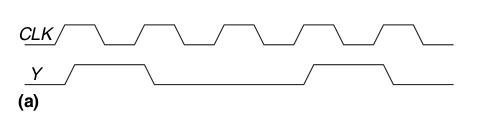
\includegraphics[width=0.8\linewidth]{./fig/fig.38a-divide-by-3-counter.png}\\
  Sketch circuit designs for such a counter
\end{prob}

\begin{prob}
  Repeat the above problem in Verilog and show a clock being reduced from 50 MHz
  to 10 Hz in ModelSim simulator. Example files covered in class,
  \href{https://vikasdhiman.info/ECE275-Sequential-Logic/lab_pdfs/pongproject-kickoff/slowclock/testslowclock.sv}{testslowclock.v}
    \href{https://vikasdhiman.info/ECE275-Sequential-Logic/lab_pdfs/pongproject-kickoff/slowclock/slowclock.sv}{slowclock.v}.
\end{prob}

{\color{red}
  Required submissions for project progress report on Nov 30 before class.
  \begin{enumerate}
  \item Modified testslowclock.sv to generate a fastclock of frequency 50MHz.
  \item Modified slowclock.sv, that outputs a slowclock of frequency 10Hz when
    the frequency of input fastclock is 50MHz.
  \item Screen shot of the waveform that you generated using ModelSim.
  \end{enumerate}
}

\subsection{Bouncing Ball}

\begin{prob}
  Design a circuit for a 1 pixel bouncing ball on a 4x4 pixel screen. You cannot design
this circuit by hand (Why?). How will you design it using Verilog? Write verilog
code and test it using a testbench?
\end{prob}

\begin{prob}
  Once you have the VGA example working, extend the above problem to 640x480
  resolution and ball represented by a box your chosen size. Connect this
  module's output to the VGA module.
\end{prob}


{\color{red}
  Required submissions for project progress report on Nov 30 before class.
  \begin{enumerate}
  \item A bouncingball.sv that bounces the ball around a screen of resolution
    640x480. The output of the module must be the 10-bit XY coordinates of the
    ball, 10-bit ballx and 10-bit bally.
  \item A testbouncingball.sv that runs at 10Hz and shows the ballx moving
    between 0 and 640 and bally moving between 0 and 480. Note that you can
    right click on wave-variable and select radix to be Unsigned decimal. You
    may use the code from Figure~\ref{lst:testbouncingball.sv} as a starting point.\\
    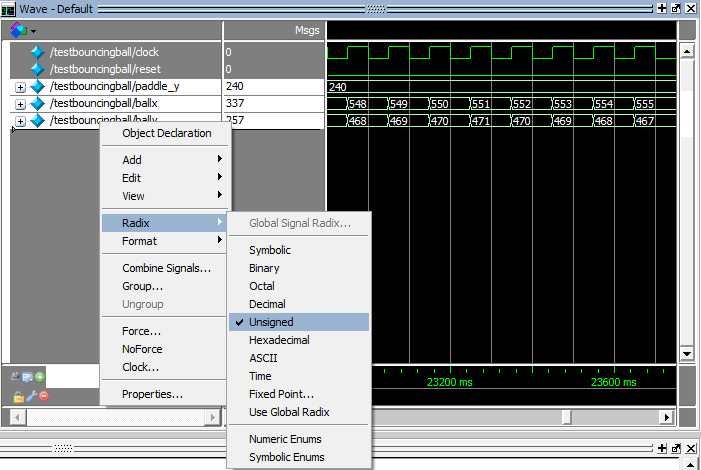
\includegraphics[width=\linewidth]{./media/testbouncingball-radix-unsigned.png}
  \item Screenshot of the waveform generated using ModelSim.
  \end{enumerate}
}

\begin{figure}
\begin{lstlisting}[language=verilog]
`timescale 10ms/1ms
module testbouncingball();
  reg clock;
  reg reset;
  reg [9:0] paddle_y;
  initial begin
    clock = 0;
    paddle_y = 10'd240;
    #5 reset = 1;
    #15 reset = 0;
  end
  always #5 clock = ~clock;
    
  wire [9:0] ballx;
  wire [9:0] bally;
  
  bouncingball bball( clock, reset, paddle_y, ballx, bally);
endmodule
\end{lstlisting}
  \caption{Sample testbouncingball.sv}
  \label{lst:testbouncingball.sv}
\end{figure}

\subsection{Moving paddle}

\begin{prob}
 Design a circuit for 1 pixel paddle on a 4x4 pixel screen. Assume that it can
 take two inputs from BUTTONs, one for moving up and another one for moving
 down. You can design this circuit by hand (Why)?
\end{prob}

\begin{prob}
  Design the above circuit using Verilog.
\end{prob}

\begin{prob}
  Once you have the VGA example working, extend the above problem to 640x480
  resolution with you
\end{prob}

{\color{red}
  Required submissions for project progress report on Nov 30 before class.
  \begin{enumerate}
  \item A paddle.sv that takes 2 bit input up\_down for up button and down
    button and outputs the Y-coordinate of the paddle which moves according to
    the button pressed.
  \item A testpaddle.sv that runs at 50Hz and shows the paddle\_y to increase and
    decreases witch change in up and down input. You
    may use the code from Figure~\ref{lst:testpaddle.sv} as a starting point.\\
    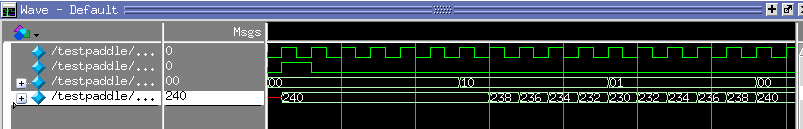
\includegraphics[width=\linewidth]{./media/testpaddle-up-down-wave.png}.
  \item Screenshot of the waveform generated using ModelSim.
  \end{enumerate}
}

\begin{figure}
\begin{lstlisting}[language=verilog]
`timescale 10ms/1ms
module testpaddle();
   reg clock;
   reg reset;
   reg [1:0] up_down; // up down buttons
   wire [9:0] paddle_y; // y coordinate of paddle y
   initial begin
      clock = 0;
      reset = 0;
      up_down = 2'b00;
      #1 reset = 1;
      #2 reset = 0;
      #10 up_down = 2'b10; // after delay of 100ms press up
      #10 up_down = 2'b01; // after delay of 100ms press down
      #10 up_down = 2'b00; // after delay of 100ms release both
   end
   always #1 clock = ~clock; // 20ms clock time period

   paddle pdl( clock, reset, up_down, paddle_y);
endmodule
\end{lstlisting}
\caption{Sample testpaddle.sv}
\label{lst:testpaddle.sv}
\end{figure}

\subsection{Ball paddle collision}

\begin{prob}
  Combine the bouncing ball problem with the moving paddle problem and bounce
  the ball only if the ball is about to hit the paddle, otherwise game is over.
  If the ball hits the paddle increment a score counter by 1.
\end{prob}


\end{document}
